%NO DATA ONLY RESULTS AND FINDINGS
\section{Introduction}

\paragraph{}
In the following sections, we will discuss our final results from two perspectives: student survey and technical. The student survey was distributed on November 2, 2021 to all applicable departments for distribution. The goal was to gain insight into what services we should offer in our final mobile library app. The technical results address the planning stages of the application development.

%----------------------------------------------------------------------------------------------------------------------------------------------
\section{Student Survey}
\paragraph{}
To best determine which services our mobile application should have, we created a campus wide survey that was distributed to the student body at WPI. The survey asked twelve thorough, yet optional, questions our team could analyze to determine current resource utilization, and to also study if those results would change if the resources were integrated within a mobile application. Would more library resources be used if they were simply easier to access? Finally, the survey also helped our team determine the demographics of the individuals who use the library resources. See Appendix 7.4 for the list of survey questions and 7.5 for the graphs of the survey results.

\paragraph{}
Of the 273 responses to our survey, 254 of them were undergraduates. That is 93\% of the total respondents (see Appendix 7.5.1)! Undergraduate students have a higher likelihood of a campus presence, compared to other academic statuses such as graduate students. Most graduate programs, WPI's included, provide more remote learning than that of undergraduate programs. Therefore the results we received came primarily from individuals who are physically on campus and interacting with the various resources at WPI. Further questions provided additional demographic data for us to analyze and gain a solid understanding of what groups of people visit the library (see Appendix 7.5.2, and 7.5.3 for those results). 

\paragraph{}
Once this analysis was completed, it was apparent that the remaining feedback in the survey would be a realistic judgement for each service under investigation. Figure 4.1 exhibits nine different library features that our team considered for possible implementation to our mobile app. The distribution in the figure pertains to the direct results from our survey. It can be seen in the graph that very few of the nine suggested services are actually utilized. Most are used only occasionally, if at all.

 \begin{figure}[H]
        \centering
        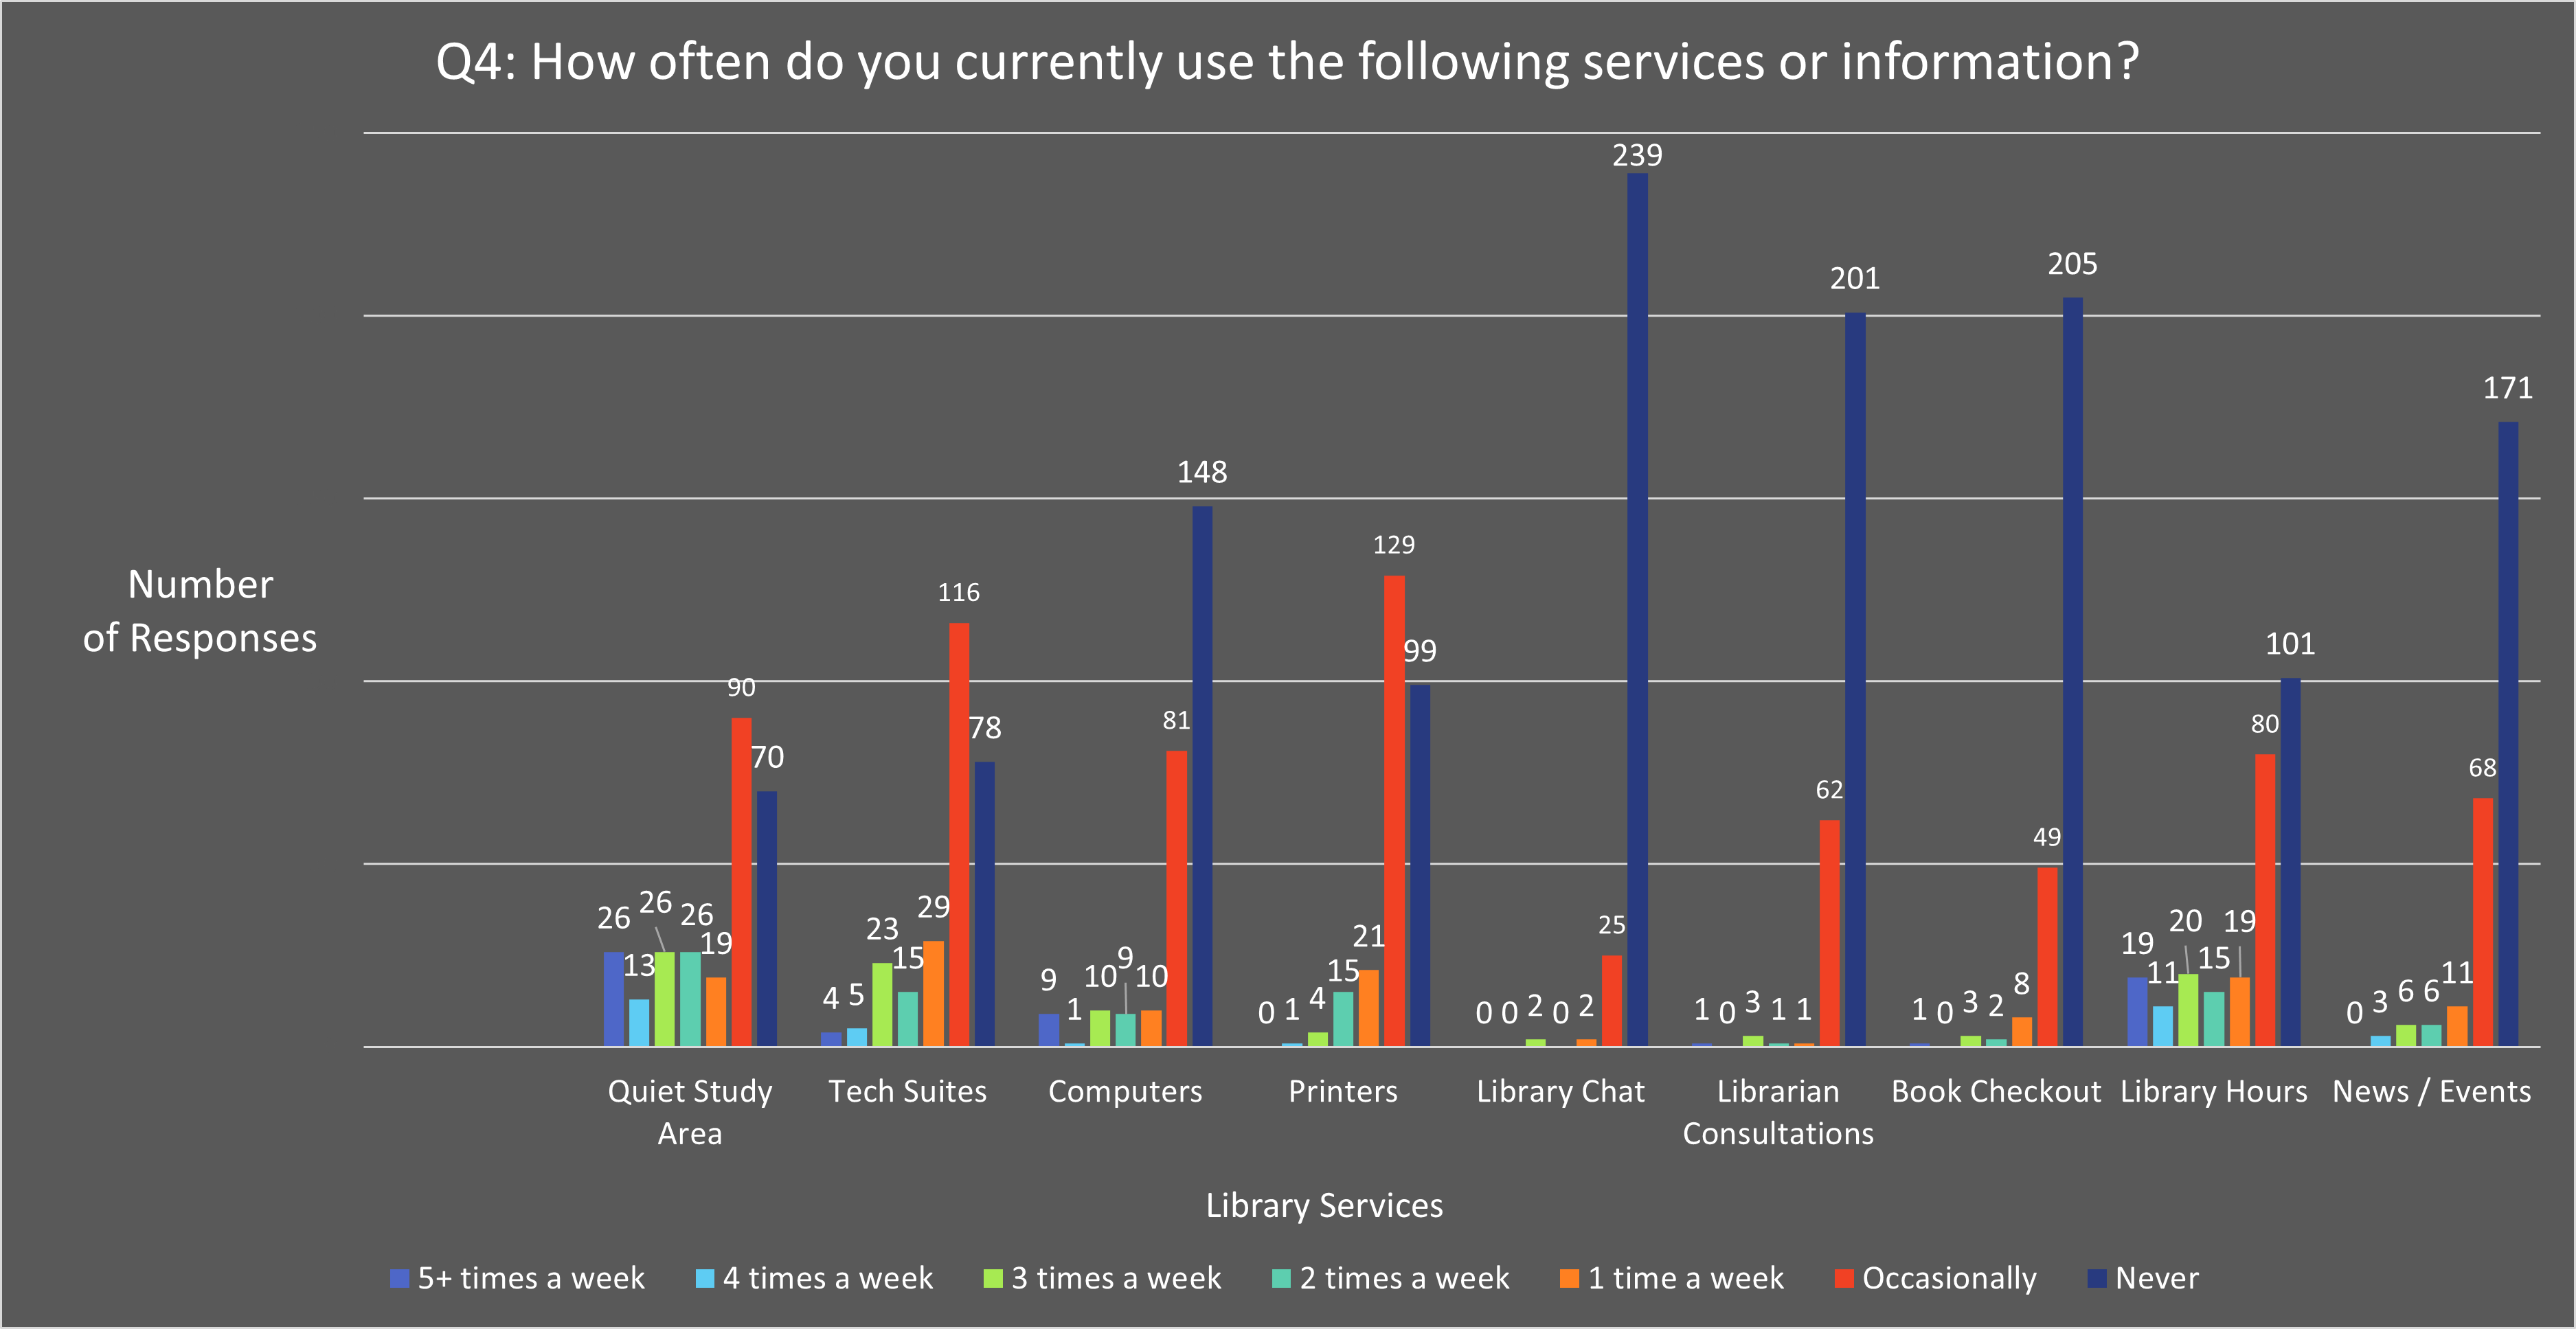
\includegraphics[width = \textwidth, height = \textheight, keepaspectratio]{assets/img/Student Survey Results Q4.png}
         \caption{Current Library Resource Usage}
    \end{figure}

\paragraph{}
In addition to this, the subsequent question in the survey simply asked whether or not the participant would use a mobile library application at all. The majority of responses were either yes or maybe. The corresponding question in the survey (see figure 4.2) provided the respondents with another, similar list of features to consider in the context of a mobile application. This encouraged them to think about which of the proposed features should be included in a mobile app for the Gordon library and which they would realistically use in such a context. This data showed that these features, in theory, would have a greater chance of being used if they were accessible through a mobile app, versus a web page or in-person usage when compared to the previous data in the previous chart.
  \begin{figure}[H]
        \centering
        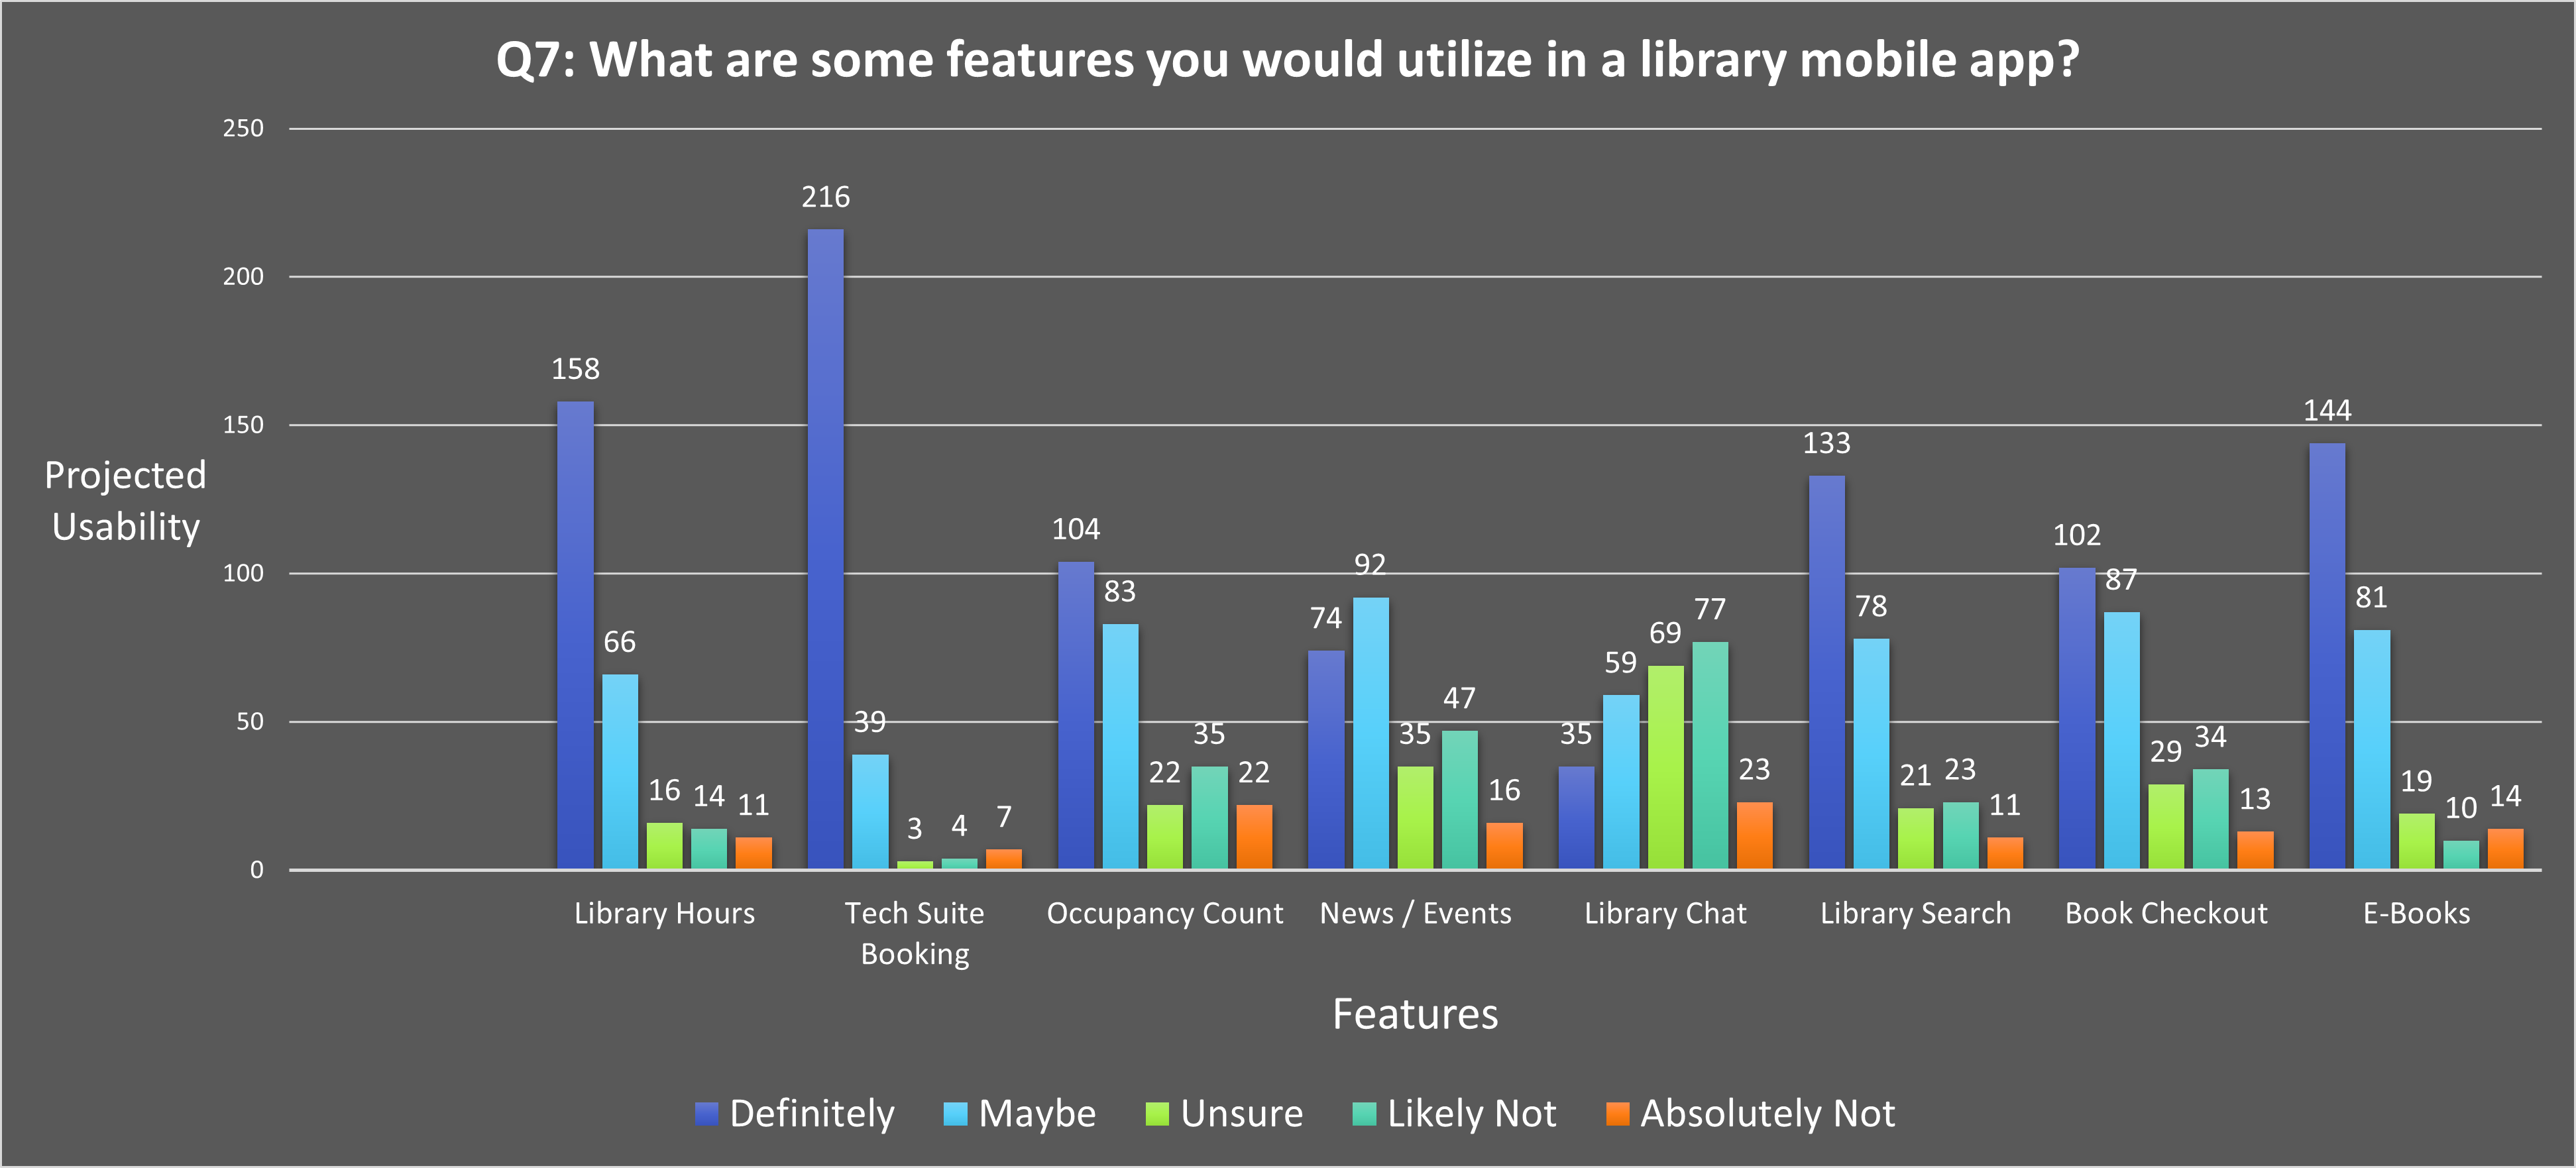
\includegraphics[width = \textwidth, height = \textheight, keepaspectratio]{assets/img/Student Survey Results Q7.png}
        \caption{Features That Might Be Used In A Mobile Environment}
    \end{figure}


\paragraph{}
 This allowed us to then narrow our list of features being considered for implementation to only five: library hours, tech suite booking, occupancy tracking, news and events, and library chat. This list was influenced by both the survey results as shown above, as well as by additional factors regarding the implementation of such features. An example of this was the potential implementation of the library search, book checkout, and e-book features. Each brought steep challenges and were beyond the scope of this project. Therefore, the list was reduced accordingly.
 
\paragraph{}
 Stepping away from the primary features of the mobile app, user interaction and flow had to be considered. Figure 4.3 shows th usage of other non-categorized mobile applications. These apps were chosen simply on the basis of popularity. 
 
 \begin{figure}[H]
        \centering
        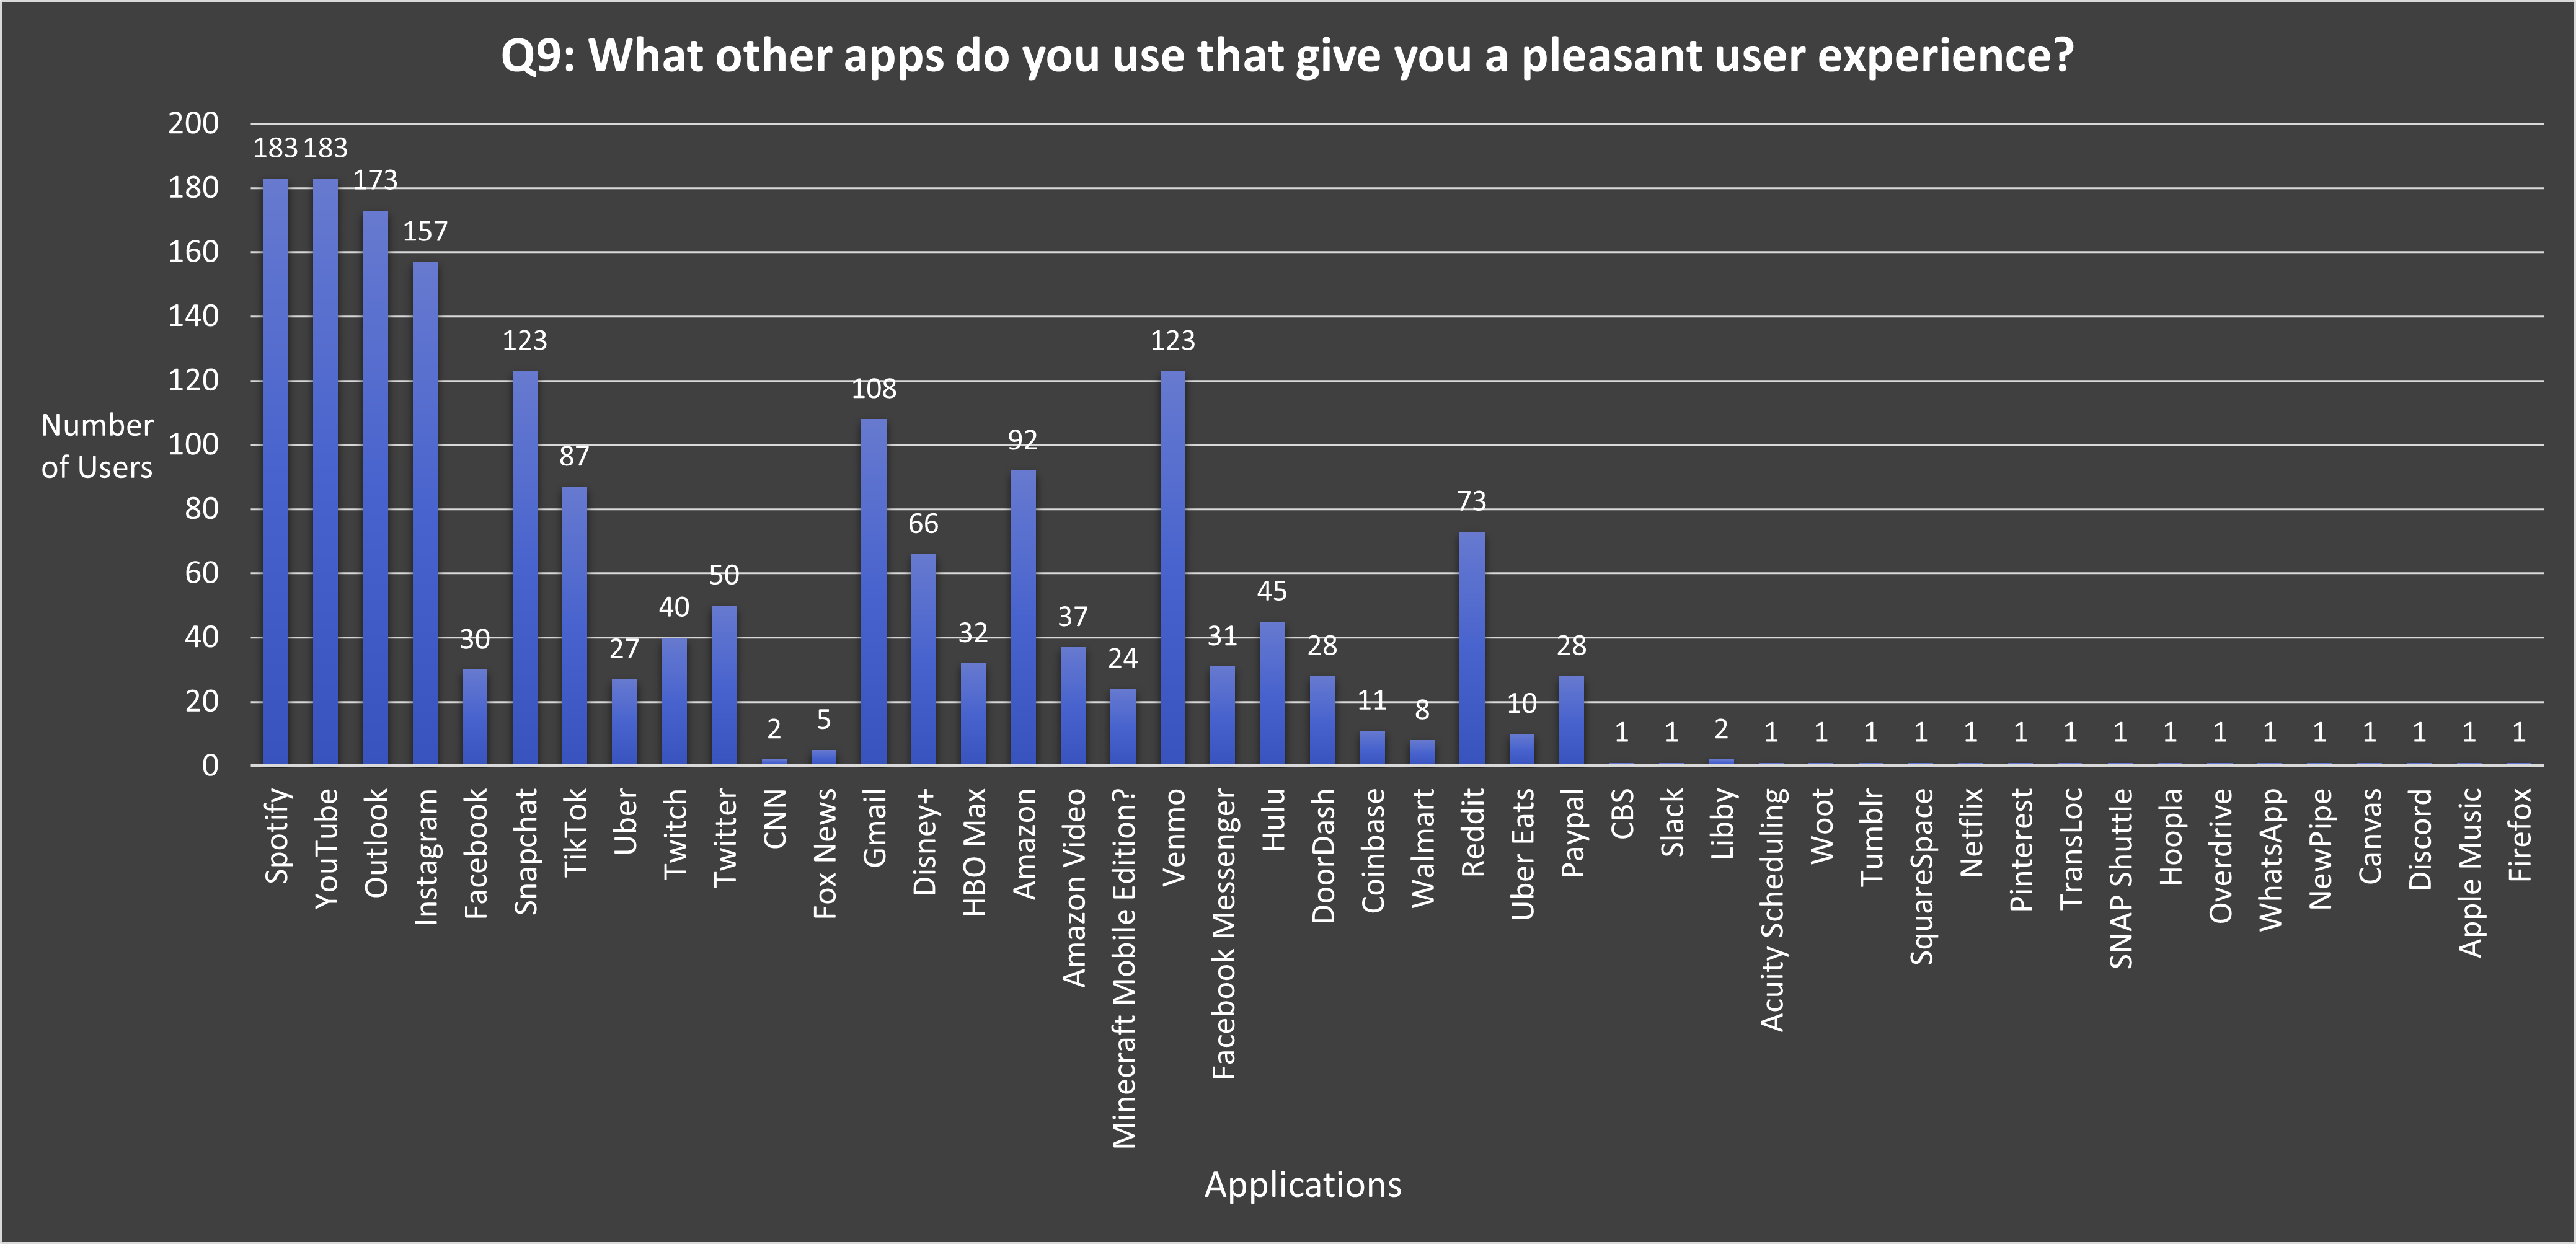
\includegraphics[width = \textwidth, height = \textheight, keepaspectratio]{assets/img/Student Survey Results Q9.png}
         \caption{User Experience Gauge}
    \end{figure}
    
The corresponding survey question allowed the participant to choose as many predetermined apps as they desired, as well as the option to provide additional apps that we did not include. Taking these results into account helped ensure that our application would follow similar modern UI (User Interface) designs like those chosen by the participants in the survey.

\paragraph{}
The final questions the respondents completed in the survey pertained to their willingness to participate as a volunteer tester for the impending prototype. Most respondents, understandably, declined their testing participation, however, 92 individuals chose to participate and 90 of them provided their academic emails for later contact regarding testing our application.

%----------------------------------------------------------------------------------------------------------------------------------------------
\section{Technical}

\paragraph{}
From a technical perspective, progress was made in the design realm. We used Figma to collaborate on these designs. Figma is a online collaborative interface design application. It enabled us to mock-up wireframes in real-time that we would then implement in code later. We began with designing a login page. Our goal was to enable users to only have to log in once, or at least not very often, as it is with various WPI single-sign-on services such as Hub and Canvas. We developed three options as pictured below. There was nothing special about the three designs specifically. We just aimed to offer ourselves some options to implement later. Seeing them helped more than describing them.

% \begin{figure}[h]
%     \centering
%     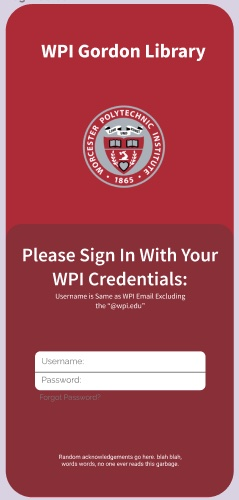
\includegraphics[width=0.25\columnwidth]{assets/img/login_1.jpg}
%     \caption{Login Screen Concept \#1}
%     \label{fig:login_1}
% \end{figure}

\begin{figure}[H]
    \centering
    \begin{subfigure}{0.33\textwidth}
        \centering
        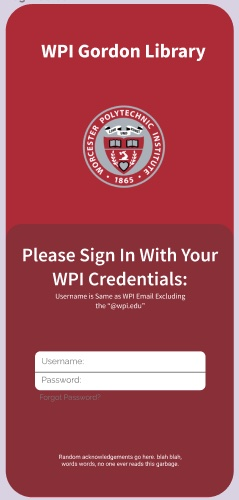
\includegraphics[width=0.6\linewidth]{assets/img/login_1.jpg}
        \caption{Design \#1}
        \label{fig:login_screens_1}
    \end{subfigure}%
    \begin{subfigure}{0.33\textwidth}
        \centering
        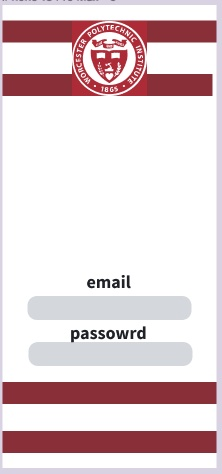
\includegraphics[width=0.6\linewidth]{assets/img/login_2.jpg}
        \caption{Design \#2}
        \label{fig:login_screens_2}
    \end{subfigure}%
    \begin{subfigure}{0.33\textwidth}
        \centering
        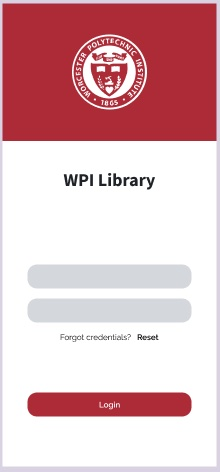
\includegraphics[width=0.6\linewidth]{assets/img/login_3.jpg}
        \caption{Design \#3}
        \label{fig:login_screens_2}
    \end{subfigure}
    \caption{Login Screen Concepts}
    \label{fig:login_screens}
\end{figure}

\paragraph{}
As the planning of the implementation progressed, we decided that a "sign-in" feature would be too cumbersome to implement in the current iteration. We moved on to designing the main page that users would see. Before receiving and reviewing the survey results, we discussed what we would like to see in the app. Considering the pandemic, we knew how important the occupancy count was, so we designed a dedicated page for it. Here are the design concepts we came up with:

\begin{figure}[H]
    \centering
    \begin{subfigure}{0.5\textwidth}
        \centering
        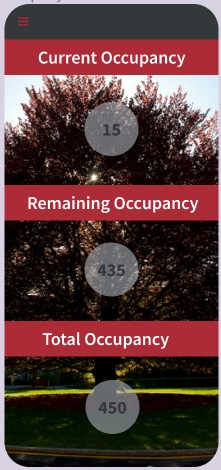
\includegraphics[width=0.6\linewidth]{assets/img/main_1.jpg}
        \caption{Design \#1}
        \label{fig:main_screens_1}
    \end{subfigure}%
    \begin{subfigure}{0.5\textwidth}
        \centering
        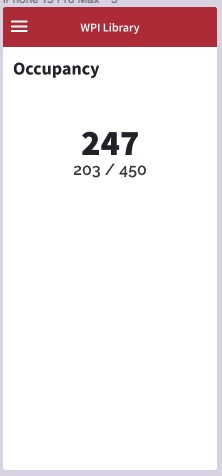
\includegraphics[width=0.6\linewidth]{assets/img/main_2.jpg}
        \caption{Design \#2}
        \label{fig:main_screens_2}
    \end{subfigure}
    \caption{Landing Screen Concepts}
    \label{fig:main_screens}
\end{figure}

\paragraph{}
Neither of these designs satisfied the goals brought forth by the survey results. From our analysis of the survey results, we determined that we would implement something similar to the right figure above, but with more features and functionality. Below the occupancy feature we wanted to embed the library's calendar in a format similar to the WPI website: \url{https://www.wpi.edu/news/calendar?og_group_ref_target_id_entityreference_filter=84091}. Based on the survey results, the feature sought after the most was tech suite booking. So, we planned for a fixed area on the bottom of the page, with a button linking to a page to book a tech suite. "Fixed," meaning that the content remains in place as the user scrolls through the page.

\paragraph{}
After we had determined the look-and-feel according to WPI standards (discussed in our Methodology), we were able to develop a style sheet and suite of reusable components that could have been used in the final product. This was Oliver's doing. He wrote dozens of CSS files and Web Components using the Lit and Vaadin frameworks.

\paragraph{}
Another technical feat was to implement a consumer for the LibCal API. This was completed through the OpenAPI specification. After given access to the LibCal platform at WPI, Oliver was able to write an OpenAPI specification of the API, which would later be used to generate client consumer code. This code would have been used by the mobile app to interact with LibCal's features, specifically so that students could book tech suites directly within the application.



%Furthermore, nearly every aspect of our mobile application was structured by the rubric displayed by modern mobile library applications and student needs to develop the best and most user-friendly application for the George C. Gordon Library and WPI alike. TAKEN FROM RESEARCH


 
%Pages: 14-18

% The Findings or Analysis Chapter: Making 
% Meaning from Your Data 
% The Findings chapter presents what you have found—the key discoveries and/or creations you have made while following your project methodology. It is sometimes called Results and Analysis, or you can give it an even more informational title specific to your project.  
% This chapter is the most important part of your entire project report!  It is where you tell what you learned about the big questions that the previous three chapters set up.   
% To think about what to include in this chapter, it is helpful to make a list of the two or three big questions at the heart of your project.  Think about the goals of the IQP: to examine the relations between science, technology, and society.  What does your project tell us about these relations?  Also, reread your introduction and background.  What is this project all about?   
 
% Content:  This chapter should not be a wholesale information dump of all of your “raw data” organized by technique (e.g., you should not have section headings of “Interview Results”, “Questionnaire Results”, etc.), but rather it should tell the reader what your data mean.  You need to process the data and decide what key findings or patterns have emerged.  In this chapter, your readers will want a SUMMARY of where you ended up and why, not every step along the way. “Analysis” may be a better word than “findings” to describe this chapter. 
% Note that the following would not be a finding: “The average yearly wind speed at the Princeton wind farm is 13.5 mph.” This would be a piece of data. The finding goes deeper and is supported by data. For example, the finding might be, “An expansion of the Princeton wind farm to two 750 kW turbines would pay for itself in eight years.” Some good questions to think about: 
% •	What were your research questions? 
% •	How did different groups of people respond to the situation you are describing? 
% •	What explains why things turned out the way they did? What evidence can you call upon? 
% •	What surprised you about the information you found? How does what you found confirm, contradict, or supplement your sources in the Background chapter?  (Be sure to bring up these sources.)  
% •	Who will be interested in your findings and why?   
% •	What do your findings tell us about the relations between technology and society? 
% It is critically important to weave in discussion about the limitations of your findings—to distinguish between what you can and can’t claim—and to acknowledge alternative interpretations and alternative viewpoints. Although it may seem counterintuitive, your work will seem more credible if you acknowledge limitations and concede some uncertainty.  Your job is not to “sell” any particular results—your job is to help the reader understand how well the results are supported by evidence. 
% A common question, related to interview results in particular, is “What belongs in the Background chapter and what belongs in the Findings chapter?”  It depends, and often there is no clear answer, but you do want to avoid repetition. If the information from the interviews provides additional background information that helps readers understand the problem your project addresses, then you probably want to include it in the Background chapter. This approach is especially common for interviews done in the first week or two of the project that provide context about local issues. However, if the information from your interviews is directly aligned with a research question posed in your Methodology chapter, then that information should be presented as evidence in the Findings chapter 
 
% Structure  
% •	Prepare the reader for your approach by writing an introductory paragraph to the chapter, prior to the first section.  The introduction of this chapter would be an overview of your findings, setting up the rest of the chapter to support those findings.  
% •	Often you can follow the same sequence of objectives or moves that you laid out in the Methodology chapter.  
% •	Depending on your findings and the nature of your project, other organizational strategies might be more effective. For example, in a project that gathers opinions from various stakeholder groups, you could arrange results according to stakeholder group if you want to emphasize those different perspectives, or you could identify themes in the results and then present the views of each stakeholder group within each of those themes.  
% •	An effective format is to state a finding in an introductory paragraph or topic sentence and then support it. It is often tempting to do the reverse, but stating the finding first generally works best for a reader. (See the sample below.) 
% •	Be careful about the amount of detail you provide.  While you should not present all of your raw data, you also need to support your claims; be sure to draw upon your data as evidence for 
% any claims that you make. For example, you could include some quotations from interviews and present summaries of your data in tables or figures.  
% •	Remember that when you include Figures and Tables, you do so to reinforce points you’re making in the narrative, not to replace narrative.  Never present a figure or table unless you refer to it in the text, explain it, and interpret it for the reader. For example: “Table 2 (not ‘The table below’) shows a summary of the results of interviews with the various stakeholder groups, divided into the areas of Strengths, Weaknesses, Opportunities, and Threats. Note that grass-roots contacts and interpersonal connections were a theme among strengths identified by both groups A and B…, whereas …” Then Table 2 should be included in the next available space following this paragraph, and the table should have a fully descriptive caption that is also included in the List of Tables and Figures following the Table of Contents at the front of the report. 
% •	If you are producing some stand-alone documents as part of your work (manual, website, or other materials), plan on placing them in an appendix.  In the Findings chapter, you would describe the findings and principles that guided the development of those documents, and point the reader to them.  The audience for those stand-alone documents is whoever will be using them.  The audience for the report is other researchers. 
 
% Example:  Following is a sample organization for a Findings chapter that illustrates some of the points above.  
% By analyzing the information gathered from our site visits and interviews, we developed the following findings concerning the tree planting projects in Heredia province, and the various stakeholders and principles which affect their success: 
% 1.	Most of the thirteen tree planting sites we visited contained trees that were correctly placed and watered, but were harmed by pests or other isolated incidents Summary of evidence, explanation, and analysis 
% 2.	Tree maintenance programs varied among the sites and the quality of tree maintenance in the private planting sites was superior to the quality of tree maintenance in the public planting sites  Summary of evidence, explanation, and analysis 
% 3.	Participation was low among business owners, developers, and the ordinary community members but was high among community leaders and schools  Summary of evidence, explanation, and analysis 
% 4.	Community members do not participate in their community’s tree planting projects because there is no confidence in the national government’s reforestation efforts, sense of ownership, or opportunity for social interactions  
% Summary of evidence, explanation, and analysis 
% 5.	There were three cases where community members were being empowered, but it appears this is not a widespread occurrence  
% Summary of evidence, explanation, and analysis 

% Features of Effective Conclusions & 
% Recommendations Chapters  
% •	Provide a succinct summary of key findings  
% •	Have directly-stated recommendations that stand out at the beginning of each paragraph or section  
% •	Use formatting that makes it easy for readers to quickly find specific conclusions and recommendations 
% •	Make clear who the recommendations are directed toward 
% •	Show consistency with Background, Methodology, and Findings chapters 
% •	Do more than recommend something; they provide a roadmap for implementation:  What methods?  What criteria should be used? What sources should be consulted? What obstacles might come up? 